%%%%%%%%%%%%%%%%%%%%%%%%%%%%%%%%%%%%%%%%%%%%%%%%%%%%%%%%%%%%%%%%%%%%%%%%%%%%%%%
% NAME:		    tree.tex
%
% AUTHOR:	    Ethan D. Twardy
%
% DESCRIPTION:	    Create a binary tree with LaTeX Tikz and PGF
%
% CREATED:	    07/31/2017
%
% LAST EDITED:	    01/01/2018
%%%
\documentclass{article}
\usepackage{tikz}
\usetikzlibrary{arrows}

\tikzset{
  treenode/.style = {align=center, inner sep=0pt, text centered, %
    font=\sffamily},
  nodesty/.style = {treenode, circle, white, font=\sffamily\bfseries, %
    draw=black, fill=black, text width=1.5em},
  nullsty/.style = {treenode, rectangle, draw=black, minimum width=0.5em, %
    minimum height=0.5em}
}

\begin{document}
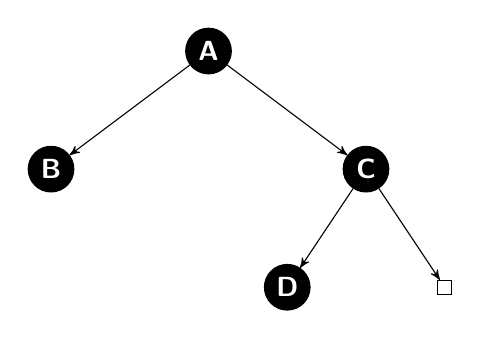
\begin{tikzpicture}[->,>=stealth',level/.style={sibling distance=4cm/#1, %
  level distance=1.5cm}]
  \node [nodesty] {A}
  child{node[nodesty]{B}}
  child{node[nodesty]{C}
    child{node[nodesty]{D}}
    child{node[nullsty]{}}
  }
  ;
\end{tikzpicture}
\end{document}

%%%%%%%%%%%%%%%%%%%%%%%%%%%%%%%%%%%%%%%%%%%%%%%%%%%%%%%%%%%%%%%%%%%%%%%%%%%%%%%
